\documentclass[10pt]{article}

\usepackage{lmodern}
\usepackage{amsmath}
\usepackage{xcolor}
\usepackage{graphicx}
\usepackage{comment}

\usepackage[style=nejm,backend=biber]{biblatex}

\usepackage{newunicodechar}
\newunicodechar{^^^^2026}{\ldots} % Mapping character: …

\usepackage{listings}
\usepackage{listingsutf8}

%% Define language for YAML
\lstdefinelanguage{YAML}{
	keywords={true,false,null,y,n},
	ndkeywords={},
	sensitive=false,
	comment=[l]{\#},
	morestring=[b]',
	morestring=[b]"
}

%% Syntax highlighting
\definecolor{codegreen}{rgb}{0,0.6,0}
\definecolor{codegray}{rgb}{0.5,0.5,0.5}
\definecolor{codepurple}{rgb}{0.58,0,0.82}
\definecolor{backcolour}{rgb}{0.95,0.95,0.92}
\lstset{
	backgroundcolor=\color{backcolour},
	commentstyle=\color{codegreen},
	keywordstyle=\color{magenta},
	numberstyle=\tiny\color{codegray},
	stringstyle=\color{codepurple},
}


\lstset{
	basicstyle=\ttfamily\footnotesize,
	%%
	%% Character encoding handling
	%inputencoding=utf8, % Not needed with UTF-8 TeX engine
	extendedchars=true,
	literate      =        % Support additional characters
		{§}{{\S}}1
		{–}{{--}}1
		{—}{{---}}1
		{…}{{$\ldots$}}1
		{→}{{\rightarrow}}1
		,
	%%
	%% Spacing
	tabsize=2,
	breakatwhitespace=false,
	breaklines=true,
	postbreak=\mbox{\textcolor{red}{$\hookrightarrow$}\space},
	keepspaces=true,
	%%
	%% Numbering
	numbers=left,
	numbersep=5pt,
	%%
	%% Space formatting
	showspaces=false,
	showstringspaces=false
	showtabs=false,
	%%
	%% Decorations
	columns=fullflexible,
	frame=single,
}

\lstdefinestyle{RvPerl}{language=Perl,
	rangeprefix=\#\#\ \{\{\ ,
	rangesuffix=\ \}\},
	includerangemarker=false,
}

\lstdefinestyle{RvSQL}{language=SQL,
	rangeprefix=--\#\#\ \{\{\ ,
	rangesuffix=\ \}\},
	includerangemarker=false,
}

\lstdefinestyle{RvR}{language=R,
	rangeprefix=\#\#\ \{\{\ ,
	rangesuffix=\ \}\},
	includerangemarker=false,
}

\lstdefinestyle{RvYAML}{language=YAML,
	rangeprefix=\#\#\ \{\{\ ,
	rangesuffix=\ \}\},
	includerangemarker=false,
}



\addbibresource{report/biblio.bib}

\begin{document}

\maketitle

\begin{abstract}
\noindent
\begin{abstractdesc}
\item[Background] TODO
%
\item[Methods] TODO
%
\item[Results] TODO
%
\item[Conclusions] TODO
\end{abstractdesc}
\end{abstract}

\tableofcontents


\section{Background}

The establishment of the clinical trial submission requirements in
Section 801 of the Food and Drug Administration Amendments Act of 2007
(FDAAA 801)~\cite{publiclaw_fdaa_2007_s801}
mandated that any applicable clinical trials (ACTs) must
submit their summary results to the \ctgov{} data bank one year from study completion.
This regulation went into effect on \ISOtoLocaleDisplayDate{2017-01-18}
and compliance was required starting 90 days later on
\ISOtoLocaleDisplayDate{2017-04-18} for all responsible
parties~\cite{ctgov_fdaaa801_final_rule_2024,zarin_trial_2016}.

\section{Methods}

\textcite{anderson_compliance_2015} present an algorithm to
determine which trials are likely to be ACTs which they term as
highly likely applicable clinical trials (HLACTs).

To ensure that similar methods are used, the replicated HLACTs
algorithm is compared against the \textcite{anderson_compliance_2015}
shared dataset~\cite{anderson_data_20130927}.

\section{Results}


\begin{figure}
	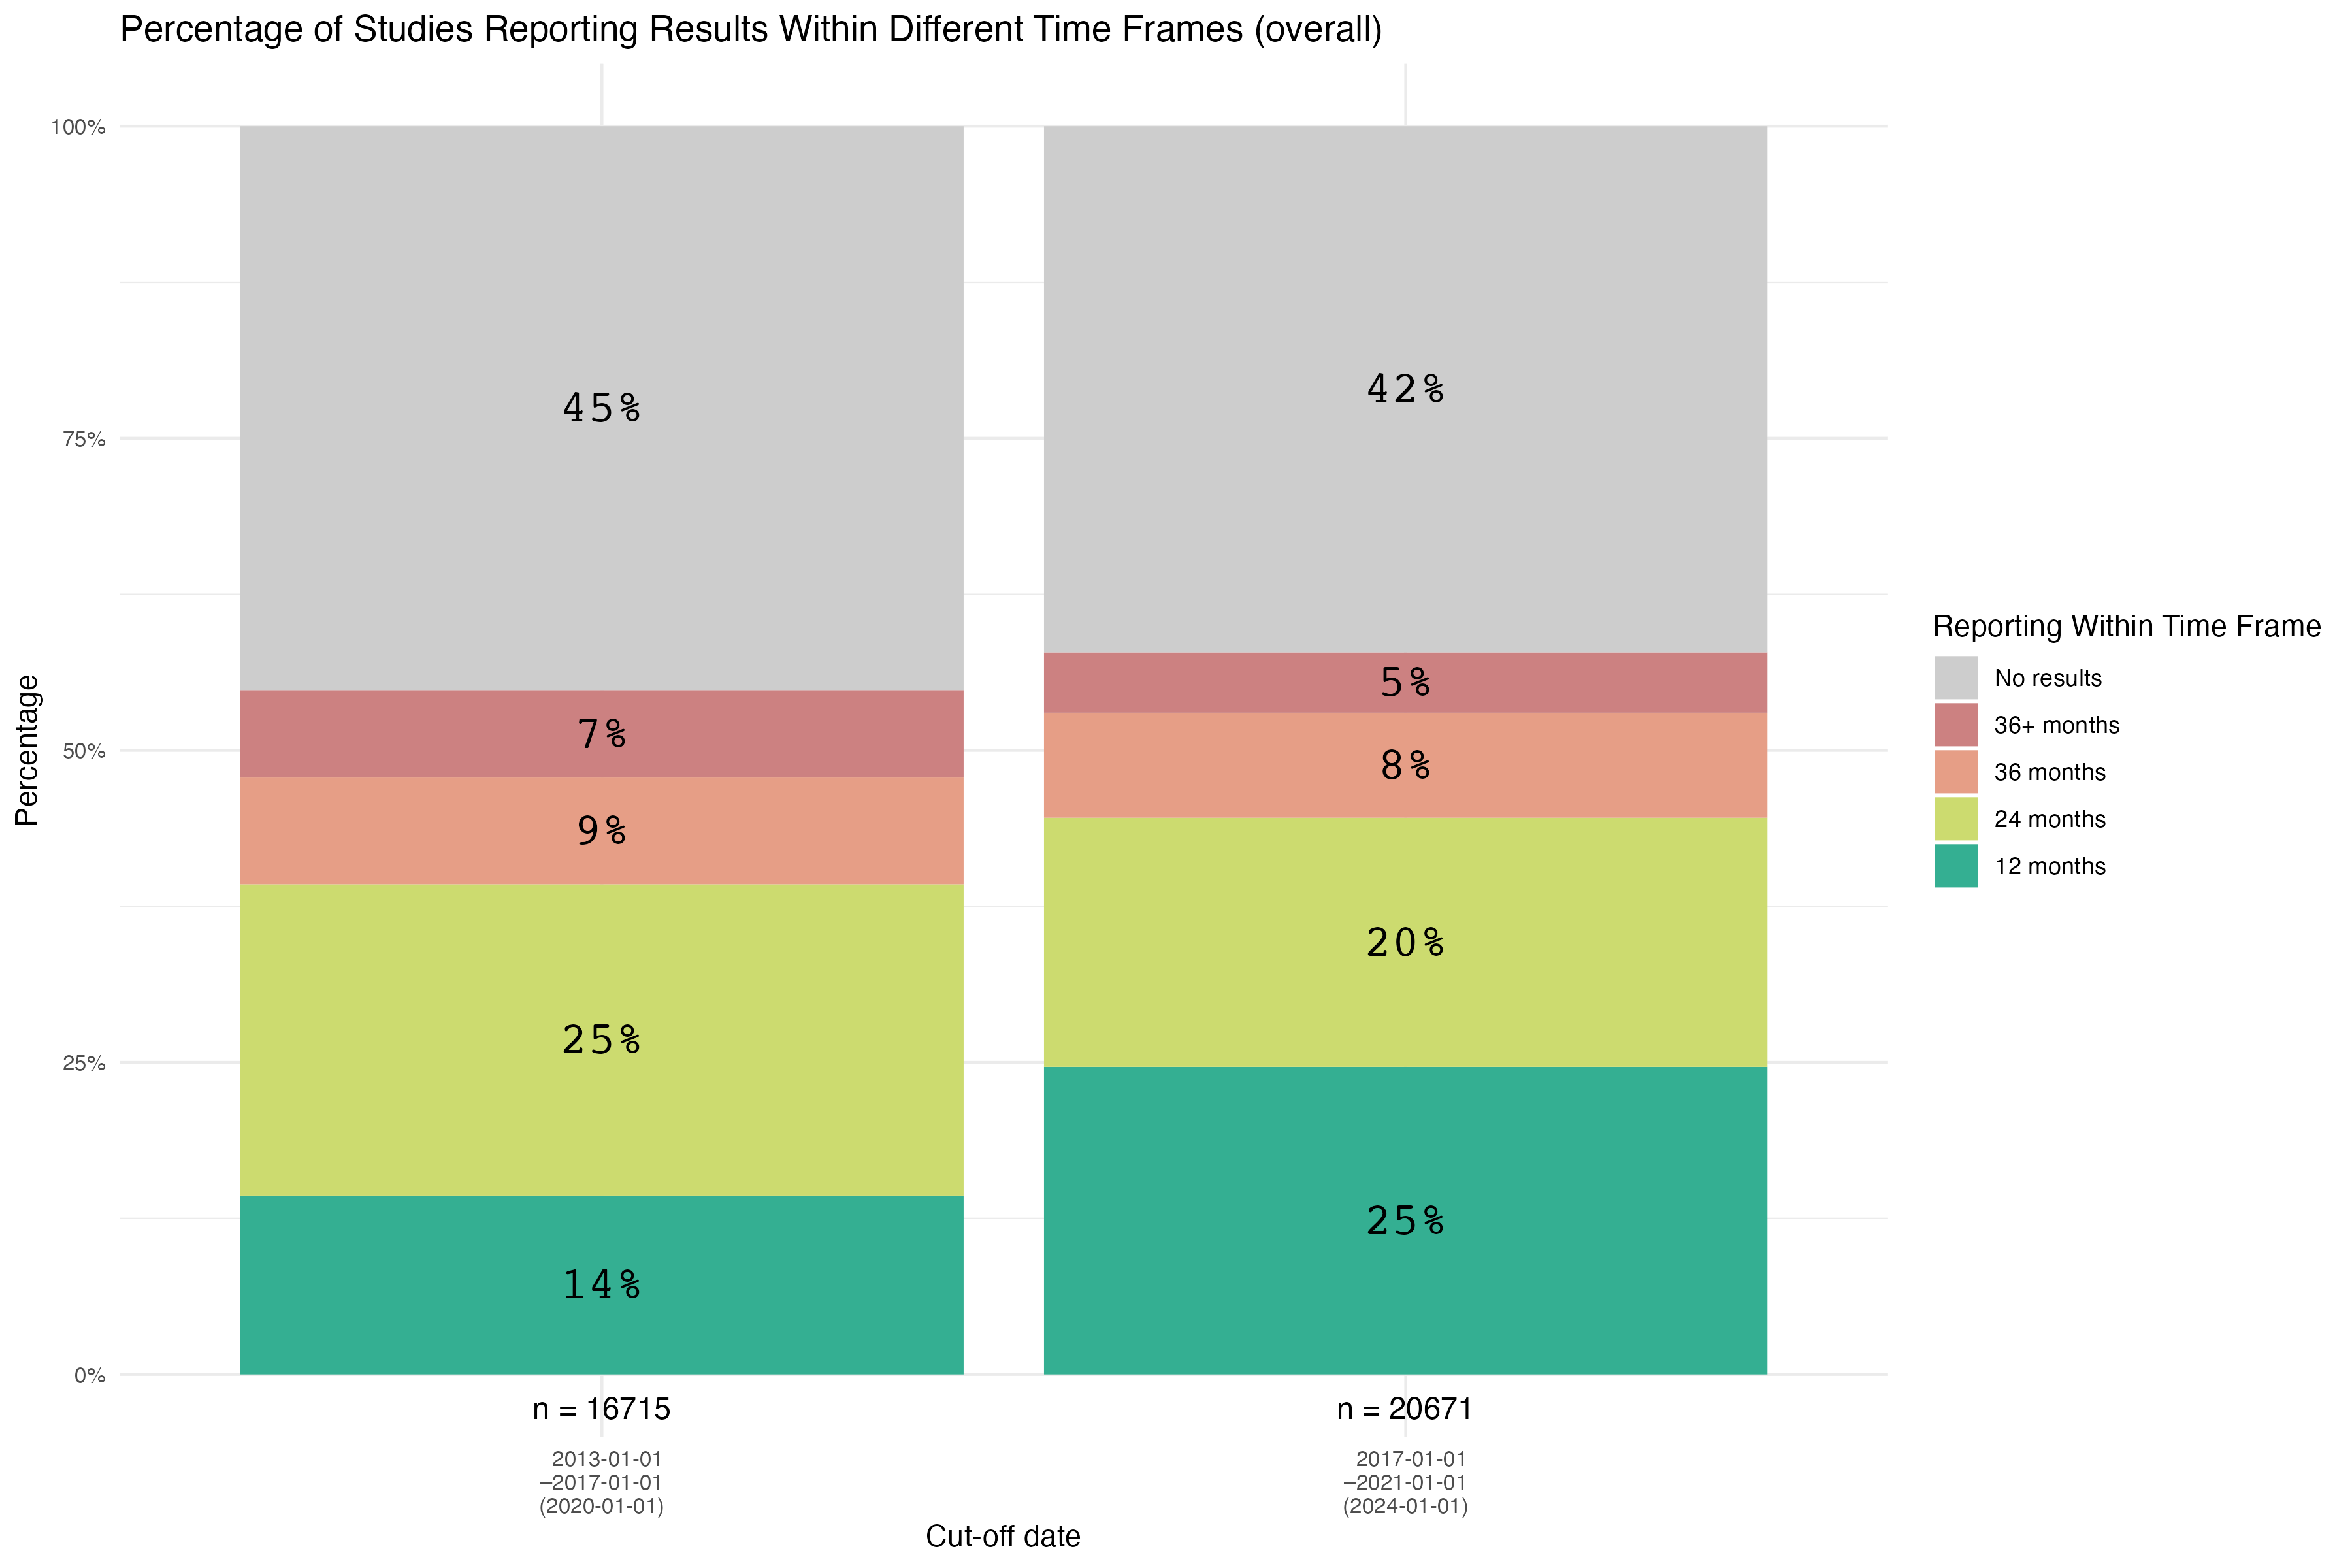
\includegraphics[width=0.95\textwidth]{figtab/rule-effective/fig.result_reported_within.facet_overall.stacked_area.png}
	\label{fig:results-reported-rule-effective-overall}
	\caption{Results before and after the effective rule date (overall)}
\end{figure}

\begin{figure}
	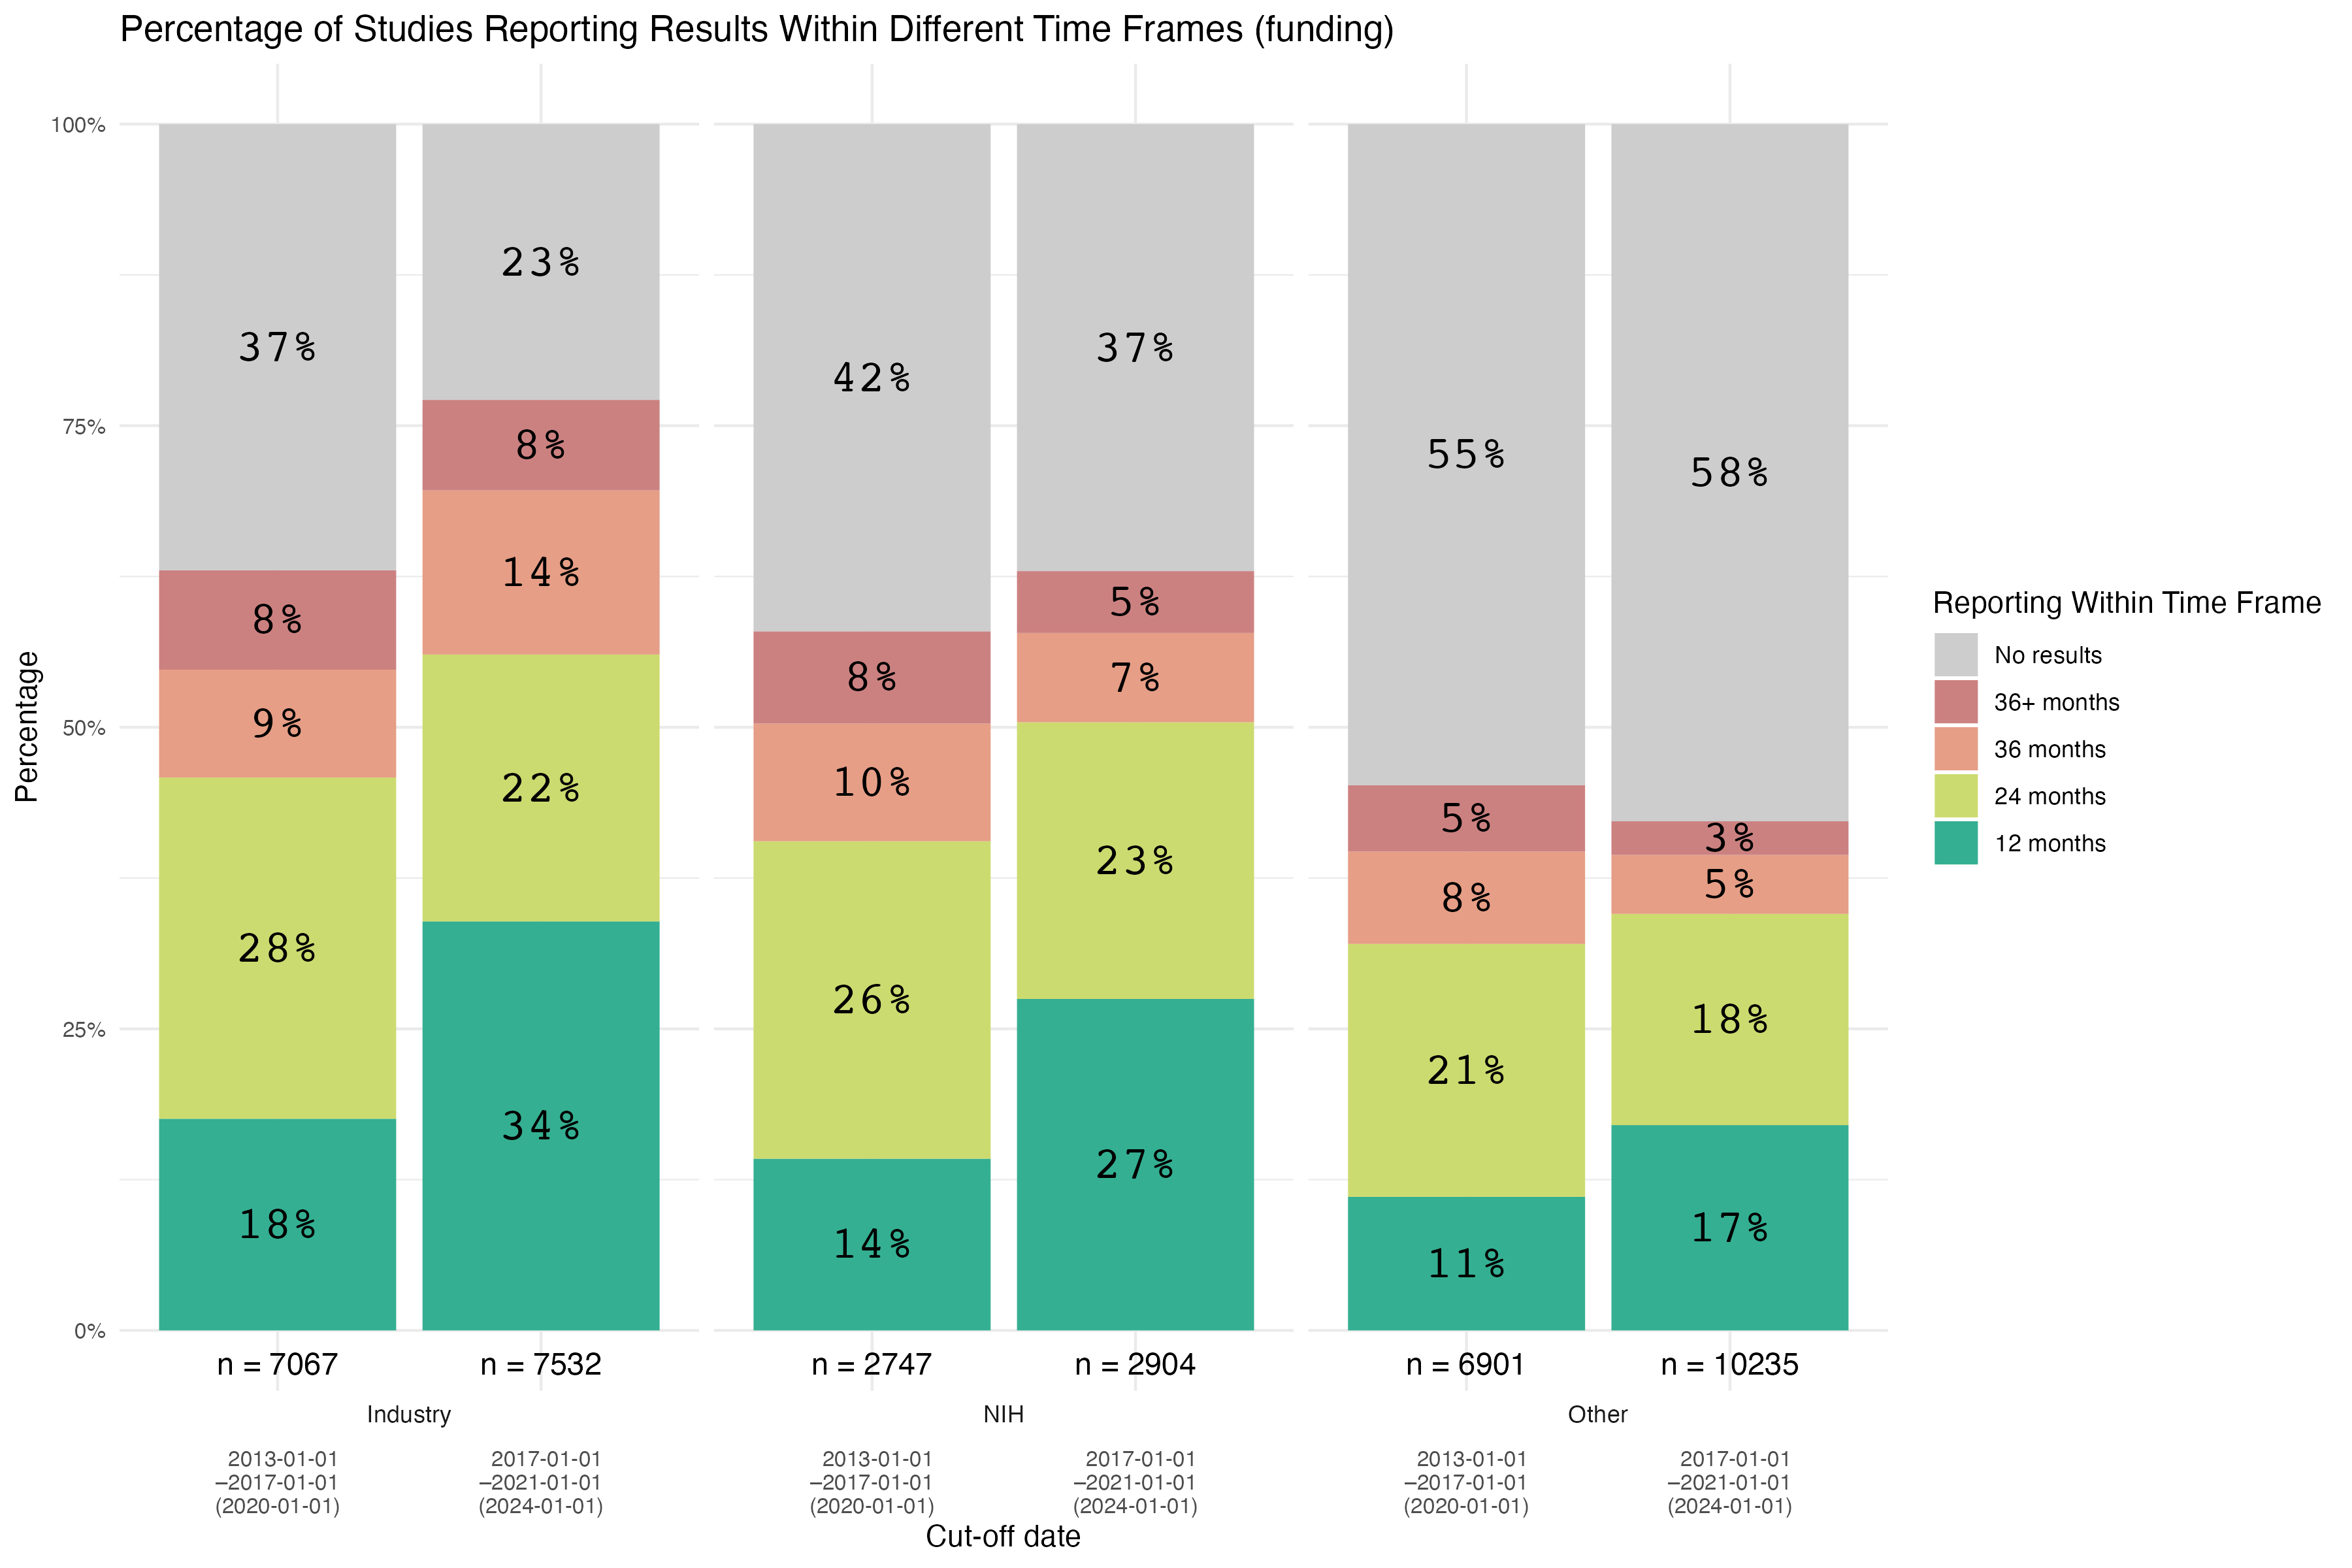
\includegraphics[width=0.95\textwidth]{figtab/rule-effective/fig.result_reported_within.facet_funding.stacked_area.png}
	\label{fig:results-reported-rule-effective-funding}
	\caption{Results before and after the effective rule date by funding source}
\end{figure}


\section{Discussion}

\printbibliography


%\section{Code review}

\subsection{Fetching data}

%\lstinputlisting[style=RvPerl,caption={Code to fetch JSONL from ClinicalTrials.gov API}]{stages/fetch-cthist-json.pl}
\lstinputlisting[style=RvPerl,
	caption={Endpoint to retrieve versions for a given NCT ID via ClinicalTrials.gov API},
	linerange=begin:ctgov_api_endpoint_version_history-end:ctgov_api_endpoint_version_history,
	%framexleftmargin=-10pt,numbersep=-8pt,xleftmargin=-12pt
]{stages/fetch-cthist-json.pl}

\lstinputlisting[style=RvPerl,
	caption={Endpoint to a particular study version via ClinicalTrials.gov API},
	linerange=begin:ctgov_api_endpoint_study_record_version-end:ctgov_api_endpoint_study_record_version
]{stages/fetch-cthist-json.pl}

\subsection{Processing \ctgov{} API data}

\begin{comment}
\lstinputlisting[style=RvSQL,caption={Process the JSONL into a Parquet file}]{sql/create_cthist_preproc.sql}
\end{comment}

\begin{comment}
\lstinputlisting[style=RvSQL,caption={Get all studies for a given cut-off date}]{sql/create_cthist_all.sql}
\end{comment}

\lstinputlisting[
	style=RvSQL,
	caption={Macro for processing funding source},
	linerange=begin:normalize_funding_source_macro-end:normalize_funding_source_all
]{sql/create_cthist_all.sql}

\lstinputlisting[style=RvSQL,
	caption={Processing location countries to determine if a trial has a US facility},
	linerange=begin:process_has_us_facility-end:process_has_us_facility
]{sql/create_cthist_all.sql}


\begin{comment}
\lstinputlisting[style=RvSQL,caption={HLACT filtering}]{sql/create_cthist_hlact.sql}
\end{comment}

\subsection{Processing for analysis}

\subsubsection{Mapping data to a common schema}

\lstinputlisting[style=RvR,
	caption={Mapping from \textcite{anderson_compliance_2015} data to common schema},
]{analysis/ctgov/preprocess/anderson2015.R}

\lstinputlisting[style=RvR,
	caption={Mapping from ClinicalTrials.gov API data to common schema},
]{analysis/ctgov/preprocess/jsonl_derived.R}

\subsubsection{Processing the common schema for further analysis}

\lstinputlisting[style=RvR,caption={Common preprocessing}]{analysis/ctgov/preprocess/common.R}

\lstinputlisting[style=RvR,
	caption={Preprocess survival},
	linerange=begin:preprocess_data.common.survival-end:preprocess_data.common.survival
]{analysis/ctgov/survival.R}

\lstinputlisting[style=RvR,
	caption={Preprocess regression},
	linerange=begin:preprocess_data.common.regression-end:preprocess_data.common.regression
]{analysis/ctgov/regression.R}

\lstinputlisting[style=RvYAML,
	linerange=begin:rule_effective-end:rule_effective
]{params.yaml}


\end{document}
